\documentclass[a4paper,11pt]{article}
\usepackage[T1]{fontenc}
\usepackage[utf8]{inputenc}
\usepackage{lmodern}
\usepackage[francais]{babel}
\usepackage{geometry}
\usepackage{graphicx}
\usepackage{amsmath}
\usepackage{amssymb}
\usepackage{mathrsfs}
\usepackage{listings,color}

\usepackage[cyr]{aeguill}


\definecolor{verbgray}{gray}{0.9}

\lstnewenvironment{code}{%
  \lstset{backgroundcolor=\color{verbgray},
  frame=single,
  framerule=0pt,
  basicstyle=\ttfamily,
  columns=fullflexible}}{}

\definecolor{shadecolor}{rgb}{.9, .9, .9}
\geometry{hmargin = 2.5cm, vmargin = 1.5cm}

\title{SY09 - TP03\\Discrimination, théorie bayésienne de la décision}
\author{Félix Flores - Cristian Garrido}
\begin{document}

\maketitle

\section{Classifieur euclidien, $K$ plus proches voisins}

%\subsection{Evaluation des performances}
Pour chacun des jeux de données, on a estimé les paramètres $ \mu_k $ et $ \sum_k $ des distributions conditionnelles,
ainsi que les proportions $\pi_k$ des classes. On a alors obtenu les résultats suivants:
\begin{enumerate}
  \item Pour le jeu de données \textit{Synth1-40}:
  \[ \pi_1  = 0.55, \pi_2  = 0.45 \hspace*{2cm} 
  \mu_1  = \begin{pmatrix}
    -1.904681 \\ 0.698841
  \end{pmatrix},
  \mu_2  = \begin{pmatrix}
    0.8808594 \\ 0.8587835
  \end{pmatrix}\]
  \[ \sum\nolimits_1 = \begin{pmatrix}
   0.7701334  & 0.2566214 \\
   0.2566214 & 1.0798685 
  \end{pmatrix},
  \sum\nolimits_2 = \begin{pmatrix}
  1.41546550  & -0.01011499 \\
  -0.01011499 & 1.22191696 
  \end{pmatrix}\]
  
  \item Pour le jeu de données \textit{Synth1-100}:
  \[ \pi_1  = 0.53, \pi_2  = 0.47\hspace*{2cm} 
   \mu_1  = \begin{pmatrix} -1.808233 \\ 1.057774 \end{pmatrix},
     \mu_2  = \begin{pmatrix} 0.9831412 \\ 1.1610775 \end{pmatrix}\]
  \[ \sum\nolimits_1 = \begin{pmatrix}
   1.50880197  & 0.07097749 \\
   0.07097749 & 0.95833356 
  \end{pmatrix},
  \sum\nolimits_2 = \begin{pmatrix}
  0.84677155  & 0.04545945 \\
  0.04545945 & 0.71631862 
  \end{pmatrix}\]  \\
  
  \item Pour le jeu de données \textit{Synth1-500}:
  \[ \pi_1  = 0.48, \pi_2  = 0.52\hspace*{2cm} 
   \mu_1  = \begin{pmatrix} -1.9101695 \\ 0.9359349 \end{pmatrix},
     \mu_2  = \begin{pmatrix} 0.9979001 \\ 0.9843533 \end{pmatrix}\]
  \[ \sum\nolimits_1 = \begin{pmatrix}
   1.16050554  & 0.03149239 \\
   0.03149239 & 0.87727376 
  \end{pmatrix},
  \sum\nolimits_2 = \begin{pmatrix}
  0.91978725  & -0.03484383 \\
  -0.03484383 & 0.95416768 
  \end{pmatrix}\] \\
  
  \item Pour le jeu de données \textit{Synth1-1000}:
  \[ \pi_1  = 0.49, \pi_2  = 0.51 \hspace*{2cm} 
    \mu_1  = \begin{pmatrix} -1.998992 \\ 1.008186 \end{pmatrix},
     \mu_2  = \begin{pmatrix} 1.0908900 \\ 0.9837324 \end{pmatrix}\]
  \[ \sum\nolimits_1 = \begin{pmatrix}
   1.03969441  & -0.07115634 \\
   -0.07115634 & 0.97107695 
  \end{pmatrix},
  \sum\nolimits_2 = \begin{pmatrix}
  1.00246869  & -0.02488749 \\
  -0.02488749 & 1.02228782 
  \end{pmatrix}\]\\
  
\end{enumerate}
On peut donc bien remarquer en tant que la taille de l'échantillon augmente les paramètres plus s’approchent à les valeurs suivantes:  
\[\pi_1 \approx  \pi_2 \approx 0.5,
\mu_1 \approx  \begin{pmatrix} -2 \\ 1 \end{pmatrix}, \mu_2 \approx  \begin{pmatrix} 1 \\ 1 \end{pmatrix}
, \sum_1 \approx  \sum_2 \approx  \begin{pmatrix}
  1  & 0 \\
  0 & 1  
\end{pmatrix}.\]


\subsection*{Estimation du taux d’erreur}
En ayant $E=\frac{1}{m}\sum 1_{z_i\ne z_i}$ alors on peut remarquer que 
   $T_i = \left\{
     \begin{array}{lr}
       1 & z_i\ne z_i\\
       0 & sinon
     \end{array}
   \right.$
suit une loi de Bernouilli, donc $T_i\sim\mathcal{\beta}(\varepsilon)$ où $\varepsilon$ représente le taux d'erreur et \[P(T_i=1)=E(E)=E(\frac{1}{m}\overset{m}{\underset{i}{\sum}}T_i)=\frac{1}{m}E(\overset{m}{\underset{i}{\sum}}{T_i})=m\overset{m}{\underset{i}{\sum}} E(T_1)=\frac{m \varepsilon}{m}=\varepsilon.\]

Puis on peut déduire que $mE$ suit aussi une loi binomiale. Maintenant on peut approcher par une loi normale en supposant que $m$ est assez grand. on a alors $mE\sim \mathcal{N}(m\varepsilon,m\varepsilon(1-\varepsilon))$.
et grâce à cela on a $E\sim \mathcal{N}(\varepsilon,m^{-1}\varepsilon(1-\varepsilon))$
Pour connaître la variance, mais on saut que on a une loi de student E : $\frac{\bar{E}-\mu}{S^*/\sqrt{N}} \sim \tau_{N-1}$. On assume les taux d'erreur $E_j$ sont indépendants. Alors On peut calculer l'intervalle de confiance pour l'espérance de E, en trouvant $\mu$,  $P(\frac{\bar{E}-\mu}{S^*/\sqrt{N}}) < 1-\alpha$
Finalement on obtient l’intervalle de confiance bilatérale suivante:
\[IC = [\bar{E} - t_{N-1;1-\alpha/2}\frac{S^*}{\sqrt{N}}, \bar{E} + t_{N-1;1-\alpha/2}\frac{S^*}{\sqrt{N}}]\]

En suite on a calculé les intervalles de confiance pour chaque jeu de donnés. En utilisant un taux d'erreur obtenu lors de vingt exécutions et avec un niveau de confiance de $1 - \alpha = 0,95$ : 
\begin{enumerate}
  \item Pour le jeu de données \textit{Synth1-40}:
  \begin{itemize}
    \item Ensemble d’apprentissage :  $\varepsilon = 0.124074$ et $IC = [0.123785,0.124363]$
    \item Ensemble de test :  $\varepsilon = 0.111539$ et $IC = [0.111250,0.111827]$
  \end{itemize}
  \item Pour le jeu de données \textit{Synth1-100}:
  \begin{itemize}
    \item Ensemble d’apprentissage :  $\varepsilon = 0.143939$ et $IC = [0.143753,0.144126]$
    \item Ensemble de test :  $\varepsilon = 0.179419$ et $IC = [0.179225,0.179598]$
  \end{itemize}
  \item Pour le jeu de données \textit{Synth1-500}:
  \begin{itemize}
    \item Ensemble d’apprentissage :  $\varepsilon = 0.122372$ et $IC = [0.122337,0.122407]$
    \item Ensemble de test :  $\varepsilon = 0.118862$ et $IC = [0.118827,0.118897]$
  \end{itemize}
  \item Pour le jeu de données \textit{Synth1-1000}:
  \begin{itemize}
    \item Ensemble d’apprentissage :  $\varepsilon = 0.104880$ et $IC = [0.104870,0.104889]$
    \item Ensemble de test :  $\varepsilon = 0.1121257$ et $IC = [0.112116,0.112135]$
  \end{itemize}
\end{enumerate}

On peut observer qu'en tant que la taille de l'échantillon augmente, l'estimation du taux d'erreur deviens au même temps plus faible. Particulièrement, dans le cas quand on a 100 individus, on a obtenu une taux d'erreur proche au dix et once percent pour l’ensemble d’apprentissage et l'ensemble de test respectivement. On peut remarquer que le taux d'erreur de l'ensemble de apprentissage et du ensemble de test est toujours approché.

\subsubsection*{Nombre optimal de voisins}

Pour obtenir le nombre optimal de voisins, on a utilisé le jeu de données \textit{Synth1-1000}, on a effectué une séparation aléatoire de l’ensemble de données en un ensemble d’apprentissage et ensemble de test; et on a comme nombre de classes candidates les valeurs 1, 2, 3, 4 et 5. Puis on a fait le test 100 fois et on a obtenu 48 fois le nombre $K=2$, 20 fois $K=5$, 14 fois $K=3$, 12 fois $K=4$ et 6 fois $K=1$. Alors on a une forte tendance au nombre de classes $K=2$. 
Cette instabilité du résultat est du à l'aléatoire. Car en dépendant les centres choisis pour l'algorithme $kmeans$ la classe à qui appartient ce centre peut varier et ceci fait changer aussi la classe à qui les points de validations appartient.
Par conséquent, on peut bien choisir comme nombre de classe optimal $K=2$.

Maintent, comme dans l'exercise précedent. on a calcule pou chaque jeu de donnés, l'estimation des taux d'erreurs et les intervalles de confiance pou l'ensamble d’apprentissage et l’ensemble de test avec un niveau de confiance de $1 - \alpha = 0,95$ : 

\begin{enumerate}
  \item Pour le jeu de données \textit{Synth1-40}:
  \begin{itemize}
    \item Ensemble d’apprentissage :  $\varepsilon = 0.082$ et $IC = [0.07826,0.081774]$
    \item Ensemble de test :  $\varepsilon = 0.132$ et $IC = [0.128227,0.131776]$
  \end{itemize}
  \item Pour le jeu de données \textit{Synth1-100}:
  \begin{itemize}
    \item Ensemble d’apprentissage :  $\varepsilon = 0.081$ et $IC = [0.080616,0.0813836]$
    \item Ensemble de test :  $\varepsilon = 0.11$ et $IC = [0.109616,0.110384]$
  \end{itemize}
  \item Pour le jeu de données \textit{Synth1-500}:
  \begin{itemize}
    \item Ensemble d’apprentissage :  $\varepsilon = 0.0694$ et $IC = [0.069330,0.069460]$
    \item Ensemble de test :  $\varepsilon = 0.0844$ et $IC = [0.084339,0.084461]$
  \end{itemize}
  \item Pour le jeu de données \textit{Synth1-1000}:
  \begin{itemize}
    \item Ensemble d’apprentissage :  $\varepsilon = 0.0557$ et $IC = [0.055672,0.055728]$
    \item Ensemble de test :  $\varepsilon = 0.0736$ et $IC = [0.073572,0.073628]$
  \end{itemize}
\end{enumerate}

On peut encore remarquer, comme dans l’exercice précédent, que en tant que la taille de l'échantillon est plus grand la différence entre le taux d'erreur pour l'ensemble d'apprentissage et celle de l'ensemble est à chaque fois plus faible.

\subsubsection*{Jeu de données Synth2-1000}

Comme l’exercice précédent, on utilise l’estimation du maximum vraisemblance pour estimer les paramètres $ \mu_k $ et $ \sum_k $,
ainsi que les proportions $\pi_k$ des classes. On a alors obtenu les résultats suivants:

  \[ \pi_1  = 0.488, \pi_2  = 0.512 \hspace*{2cm} 
    \mu_1  = \begin{pmatrix} -4.055942 \\ 1.011496 \end{pmatrix},
     \mu_2  = \begin{pmatrix} 4.028957 \\ 1.067821 \end{pmatrix}\]
  \[ \sum\nolimits_1 = \begin{pmatrix}
   1.014560  & 0.018451 \\
   0.018451 & 0.939754 
  \end{pmatrix},
  \sum\nolimits_2 = \begin{pmatrix}
  4.953398 & 0.107909 \\
  0.107909 & 5.022125 
  \end{pmatrix}\]\\

  En approximant ces valeurs on peut les estimer comme:
\[\pi_1 \approx  \pi_2 \approx   0.5,
  \mu_1 \approx  \begin{pmatrix} -4 \\ 1 \end{pmatrix}, \mu_2 \approx  \begin{pmatrix} 4 \\ 1 \end{pmatrix}
, \sum_1 \approx  \begin{pmatrix}
  1  & 0 \\
  0 & 1
  \end{pmatrix}
, \sum_2 \approx  \begin{pmatrix}
  5  & 0 \\
  0 & 5  
\end{pmatrix}\].\\\\  

Maintenant on calcule l'estimation des taux d'erreur avec les deux classificateurs.

\begin{enumerate}
  \item Avec classificateur de distance euclidienne:
  \begin{itemize}
    \item Ensemble d’apprentissage :  $\varepsilon = 0.0063063$ et $IC = [0.006305,0.006308]$
    \item Ensemble de test :  $\varepsilon = 0.006587$ et $IC = [0.006585,0.006588]$
  \end{itemize}
  \item Avec classificateur de plus proche voisin:
  \begin{itemize}
    \item Ensemble d’apprentissage :  $\varepsilon = 0.0047$ et $IC = [0.004697,0.004703]$
    \item Ensemble de test :  $\varepsilon = 0.0066$ et $IC = [0.006597,0.006603]$
  \end{itemize}
\end{enumerate}

Après ce calcule, on peut noter que les estimations obtenus sont beaucoup plis fiables. Cela principalement du à la grande quantité de donnés et surtout parce que les variances entre les classes son beaucoup plus distantes par rapport aux jeux de donnés précédant. Ce fait alors avoir des centres plus éloignés et donc par le deux classificateurs un tirage plus forte par les classes.

\pagebreak


\section*{Règle de Bayes}

\subsection{Distributions marginales des variables $X_1$ et $X_2$ dans chaque classe}

Car les matrices de covariance ($\Sigma_1$ et $\Sigma_2$) sont diagonales, on peut déduire que les variables $X_1$ et $X_2$ sont indépendants. Par ailleurs, les données qui appartient à chaque classe $\omega_1$ et $\omega_2$ suivent une loi normal bivariée.
Aussi, les vecteurs aléatoires suivent aussi une loi normal, de coup on peut encore remarquer que les composants de $X_1$ et $X_2$ suivent une loi normal.
\[X_1 \sim \mathcal{N}(\mu_{1}, 1)\]
\[X_2 \sim \mathcal{N}(\mu_{2}, 1)\]


\subsection{Courbes d’iso-densité.}

Si on analyse l’équation de la courbe d’iso-densité de la classe 1 et la classe 2, on a :\\
$(x - \mu_1)^t\sum_1^{-1}(x-\mu_1)=c_1$  (pour la classe 1) et 
$(x - \mu_2)^t\sum_2^{-1}(x-\mu_2)=c_2$ (pour la classe 2), où $c_1$ et $c_2$ sont constants.
En plus, on sait que $\Sigma_1$ et $\Sigma_2$ sont matrices identité. Donc, les courbes d'iso-densité ont l'équation suivante:
\[(x-\mu_1)^t(x-\mu_1) = c_1, (x-\mu_2)^t(x-\mu_2) = c_2\]

En fin, on peur conliure que les centres des cercles sont $\mu_1$ et $\mu_2$ et ses rayons sont donnés par $\sqrt{c_1}$ et $\sqrt{c_2}$ .


\subsection*{Règle de Bayes}
Règle de Bayes :
$\delta^{*}(x) =
\begin{cases} 
  a_{1} & si \frac{f_{1}(x)}{f_{2}(x)} > \frac{\pi_{2}}{\pi{1}} \\
  a_{2} & sinon.
\end{cases}$\\ \\


Après des simplifications, on peut écrite la règle de Bayes comme l'expression suivante: 
\[\delta^{*}(x) = \begin{cases} 
  a_{1} & si  \> x_1 < \frac{ln(\pi_1)-ln(\pi_2)}{3} - \frac{1}{2} \\
  a_{2} & sinon.
\end{cases}\]

Si on considère que $\pi_1 = 0.5$ donc $\pi_2= 0.5$ pour lex jeux de données $Synth1-40, Synth1-100, Synth1-500$ et $Synth1-1000,$ et en remplaçant ces valeurs dans l'équation au dessus, on obtient finalement l'équation suivante:
\[\delta^{*}(x) = \begin{cases} 
  a_{1} & si  \> x_1 < - \frac{1}{2} \\
  a_{2} & sinon.
\end{cases}\]



\subsection*{Frontières de décision}

Ci-dessous, on montre les graphiques correspondantes aux jeux de données $Synth1-40, Synth1-100, Synth1-500$ et $Synth1-1000,$ pour le problème de discrimination des classes $\omega_{1}$ et $\omega_{2}$ :
\begin{center}
  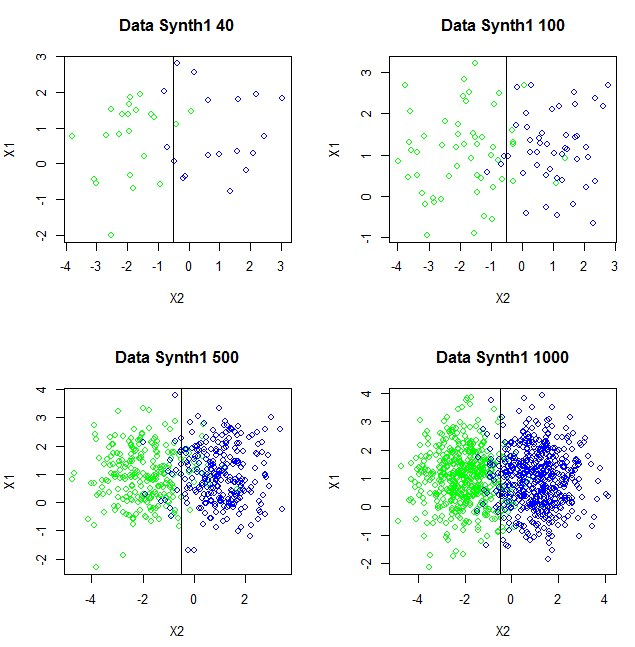
\includegraphics[height = 15cm, width = 15cm]{data.jpg}
\end{center}


On peut remarquer dans la graphique de $Synth1-40$ et $Synth1-100$ que est difficile de faire une distinction de classes donné le cas dont n'existe pas la troisième colonne (colonne de classe). Néanmoins, pour les jeux de données $Synth1-500$ et $Synth1-1000$ (spécialement pour $Synth1-1000$) on peut déjà noter un centre plus consistent et une nuage de données plus concentrée autour de chaque classe. 



\subsection*{Erreur de Bayes}

Pour obtenir une perspective mathématique de l'erreur de Bayes appliqué aux jeux de donnés $Synth1-40, Synth1-100, Synth1-500$ et $Synth1-1000,$ on doit calculer ses estimateurs (Estimateur $\alpha$ et $\beta$).
Les fonctions de ces estimateurs sont ajoutés dans l'annexe de ce rapport.


\[
\begin{tabular}{|c|c|c|}
\hline
 & $\alpha$ & $\beta$ \\
\hline
Synth1-40 & 0.09090909 & 0.09090909 \\
\hline
Synth1-100 & 0.1320755 & 0.05660377 \\
\hline
Synth1-500 & 0.08333333 & 0.07083333 \\
\hline
Synth1-1000 & 0.07786885 & 0.05737705 \\
\hline
\end{tabular}
\]
\pagebreak

\section*{ANNEXES}
      \begin{code}
      ceuc.val <- function(mu, Xtst){
	      ntst = dim(Xtst)[1];
	      ptst = dim(Xtst)[2];
	      Ztst = NULL;
	
	      h.x <- rowSums(Xtst^2)
	      h.y <- rowSums(mu^2)
	      ones.n <- rep(1,ntst)
	      ones.m <- rep(1,dim(mu)[1])
	      D2 <- h.x\%*\%t(ones.m) - 2*as.matrix(Xtst) \%*\% t(mu) + ones.n\%*\%t(h.y)
	      for(k in 1:ntst){
		      pproche = min(D2[k,]);
		      Ztst = c(Ztst,as.numeric(rownames(mu)[which(pproche == D2[k,])]))
	      }
	      Ztst;
      }
      \end{code}
      
      \begin{code}
      ceuc.app <- function(Xapp, zapp){
	      g <- max(zapp)
	      muk = NULL;
	      for(k in 1:g){
		      indk = which(zapp==k);
		      rw = t(as.matrix(apply(Xapp[indk,],2,sum)/dim(Xapp[indk,])[1]));
		      rownames(rw) = k;
		      muk = rbind(muk,rw);
	      }
	      muk;
      }
      \end{code}
      
      \begin{code}
      kppv.val <- function(Xapp, zapp, K, Xtst)
      {
        centers = cbind(kmeans(Xapp,K)$centers,rep(Inf,K));
        X = cbind(Xapp,zapp);
        for(i in 1:nrow(centers)){
          centers[i,3] <- getClass(X,centers[i,1:2])
        }
        print("Centers:")
        print(centers)
        Ztst = NULL;
        for(i in 1:nrow(Xtst)){
          Ztst = rbind(Ztst,getClass(centers,Xtst[i,]))
        }
        Ztst;
      }

      getClass <- function(X,p){
        d = Inf;
        cl = NULL;
        for(i in 1:nrow(X)){
          disPto = dist(rbind(X[i,1:2],p));
          if(d > disPto){
            d = disPto;
            cl = X[i,3];
          }
        }
        cl;
      }
      \end{code}

      \begin{code}
      kppv.app <- function(Xapp, zapp, Xval, zval, nppv)
      {
        Kideel = NULL
        max = 0;
        for(K in nppv){
          zppv = as.vector(kppv.val(Xapp,zapp,K,Xval))
          print(sum(zppv == zval))
          if(sum(zppv == zval) > max){
            Kideel = K
            max = sum(zppv == zval);
          }
        }
        Kideel
      }
      \end{code}
      
      \begin{code}
      estimateurAlpha <- function(data){
        f<-function(row) {
          if(row[3] == 1 && row[1] > -0.5){ 
            return(1) 
          } 
          return(0) 
        }
        sum(apply(data, 1,f )) / sum(data[,3] == 1)
      }
      
      estimateurBeta <- function(data){
        f <- function(row) {
          if(row[3] == 2 && row[1] < -0.5){ 
            return(1) 
          } 
          return(0) 
        }
        sum(apply(data, 1, f)) / sum(data[,3] == 1)
      }
      \end{code}

\end{document}
